%************************************************
\chapter{Introduction}\label{ch:introduction}
%************************************************

\section{Preliminary Definitions and Assumptions}

\subsection{Multi-agent systems \& Intelligent Agents}\label{sec:agents}

The term \ac{MAS} is a broad term encompassing an array of different concepts and applications. While the meaning of the term can be decomposed to be a system of multiple agents, the definition of an agent remains to be settled~\citep{Wooldridge2002}. There is some consensus that, firstly agents are computer systems situated in an environment, and that they are autonomous. Other important features of agency are given as~\citep{Wooldridge1995,HayesRoth1995}:
\begin{itemize}
\item \emph{reactivity}---agents perceive their environment, including other agents, and react to changes in it.
\item \emph{proactivity}---agents are able to exhibit goal-directed behaviour.
\item \emph{communication}---agents can have some kind of social capacity to interact with other agents.
\end{itemize}

Thus the requirements for agency are tied to both the capabilities of system, and the way in which it makes decisions (in contrast to agency in social sciences which only requires autonomy). These requirements act as a way of excluding basic systems, such that not all systems and programs would be classified as agents~\citep{Franklin1997}.

When in an environment, an agent reads the state of the environment via sensors, and performs actions to change the state of the environment. In most cases the control that the agent can exert on the environment will only be partial, in that it can influence the state of the environment. The effect of an action may not be deterministic, or it may not have any affect at all, depending on the properties of the environment~\citep{Wooldridge2002}.

The properties of an environment can be classified according to several relevant criteria~\citep[p.46]{Russell2003}:
\begin{itemize}
\item \emph{Accessible}---If an agent can perceive the complete environment state via its sensors, then the environment is accessible to this agent.
\item \emph{Deterministic}---If the next state of the environment is determined purely from the current state and actions of agents, then it is deterministic.
\item \emph{Episodic}---In an episodic environment the quality of actions do not depend on previous actions.
\item \emph{Static} or \emph{dynamic}---If the environment can change while an agent is deciding on an action then the environment is dynamic for the agent; otherwise it is static.
\item \emph{Discrete} or \emph{continuous}---If the set of possible environment states is finite, then the environment is discrete; otherwise it is continuous.
\end{itemize}

\citet[pp.31--32]{Wooldridge2002} provides a formalisation of an abstract \ac{MAS}. This defines a \emph{run} of an agent in an environment as a sequence of interleaved environment states and actions, representing the history for that agent; a \emph{state transformer} function which defines the effect that agents actions have on the environment state; and an \emph{agent function} which maps a \emph{run} for an agent to an action, representing an agent's decision process.

\section{Methodology}

In this thesis we follow closely a methodology called \ac{SIC}~\citep{Jones2013}. This is a method for the design of socio-technical systems from the analysis of social and organisational concepts. Built upon the synthetic method underlying research in artificial societies and artificial life~\citep{Steels1994}, the formalisation of social relations in multi-agent systems~\citep{Neville2004}, and other attempts to apply ideas from the social sciences to the design of computational systems~\citep{Edmonds2005}, it provides a series of steps to go from an observed social phenomenon to an observed performance of a derived computer model under controlled experimentation conditions. These steps are illustrated in \autoref{fig:sic}.

\begin{figure}
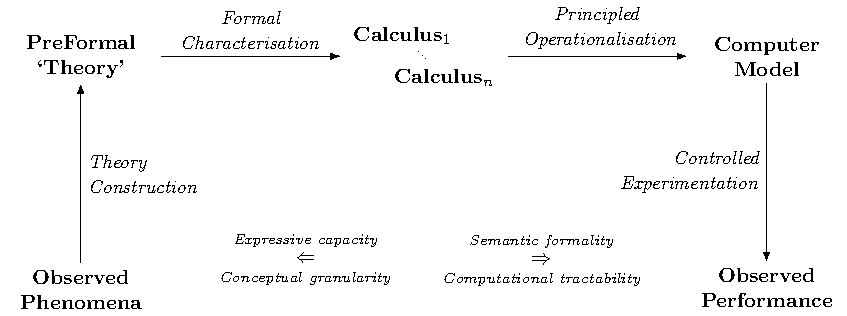
\includegraphics[width=\linewidth]{gfx/sic}
\caption[Methodology for sociologically inspired computing.]{Methodology for sociologically inspired computing~\citep{Jones2013}.}\label{fig:sic}
\end{figure}

% TODO Interleave what we actually do.
We begin with an observed phenomenon, for example, from the social sciences, a human social, legal, or organisational system. The process of \emph{Theory Construction} generates a \emph{PreFormal Theory}, usually expressed in a natural language. \emph{Formal Characterisation} creates a specification of this theory in a calculus of some kind, where `calculus' is meant to be any system of calculation or computation based on the manipulation of symbolic representations. This calculus is then embedded in a computer model in the \emph{Principled Operationalisation} step. This computer model enables simulations that can include both implementations of individual agents, and/or treatment of large populations. Through \emph{Controlled Experimentation} with this computer model we can observe the performance of the model.

Through our use of this methodology we have two major contributions to the \emph{Principled Operationalisation} and \emph{Controlled Experimentation} steps. The platform Presage2~\citep{Macbeth2014} which enables both of these steps, and a rule engine for Electronic Institution which enables rapid operationalisation of common concepts from Electronic Institutions, with flexibility to accommodate further rules from the calculus. These contributions are presented in \autoref{ch:presage} and \autoref{ch:droolseinst} respectively.
